\documentclass[11pt,mathserif]{beamer}
\usepackage[utf8]{inputenc}
\usepackage[english]{babel}
\usepackage{tikz}
\usepackage{amsmath,amssymb,mathtools}
\usepackage{tensortyping}
%\usepackage{movie15}
\usepackage{multimedia}
%\usepackage[]{biblatex}

\usepackage{pgfplots}
\usepgfplotslibrary{patchplots}
\usepgfplotslibrary{groupplots}
\pgfplotsset{compat=1.3}

\newcommand{\roughcite}[1]{\textit{#1}}

\usetheme[titlepagelogo=Avancez_black.pdf,titleflower]{chalmers}

% Some some front page information
\title{Multiscale Modeling of Sintering of Hard Metal}
%\subtitle{And something more}
\author{Mikael Öhman}
\institute{Chalmers University of Technology}
% Bibliography
%\bibliography{references_extended}

\begin{document}

\section{Title page}
\begin{frame}[plain]
 \titlepage
\end{frame}

\section{Outline}
\begin{frame}
 \frametitle{Outline}

\begin{itemize}
 \item Background
 \item Sintering phenomena on mesoscale
 \item Surface tension
 \item Multiscale modeling
 \item OOFEM: Object Oriented Finite Element Method
 \item Future work
\end{itemize}
\end{frame}

\section{Background}
\begin{frame}
 \frametitle{Project background and motivation}
 \begin{itemize}
  \item Complicated macroscopic constitutive models
  \begin{itemize}
    \item Many parameters, impossible to measure
    \item Needs experimental calibration
  \end{itemize}
  \item Computational power increasing
 \end{itemize}

 \roughcite{Mähler, Ekh \& Runesson (1999)}

 \roughcite{Svoboda \& Reidel  (1996)}
\end{frame}

\subsection{Sintering}
\section{Sintering}
\begin{frame}
 \frametitle{Sintering phenomena on the mesoscale}

% The sintering phenomenon on the mesoscale is driven by surface tension on the melted binder, and
% the homogenized effect of the surface tension is the so-called sintering stress.
% From the macroscopic perspective, the specimen (green body) shrinks due to this volumetric sintering stress. In the case of inhomogeneous
% initial density in the green body, the sintering can result in unwanted final deformations.

 \begin{enumerate}
  \item Mixture of WC and Co particles (micrometer size)
  \item Heating and softening of binder
  \item Melting binder
  \item Bridging between particles
  \item Particles aggregate
  \item Compaction due to surface tension
 \end{enumerate}
\begin{center}
 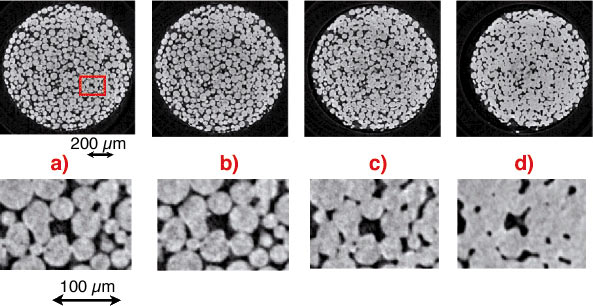
\includegraphics[width=0.6\textwidth]{figures/fig081.jpeg}
\end{center}
\end{frame}

\begin{frame}
 \frametitle{Modeling of sintering on the mesoscale}

 \begin{itemize}
  \item Incompressible Stokes flow problem
  \item Finite element
  \begin{itemize}
    \item Taylor-Hood element
    \item Surface tension element
  \end{itemize}
  \item Explicit time stepping
  \item Updated Lagrangian formulation
  \item Simple constitutive driver
 \end{itemize}

\begin{figure}[hbpt]
 \centering
 \begin{tikzpicture}
  \begin{groupplot}[
    group style={group size=3 by 1},
    width=4cm,
    height=4cm,
    xticklabels={},
    yticklabels={},
    %colormap/cool,
    patch to triangles,
    %patch refines=1,
	%shader=interp,
	%shader=flat,
    %colorbar style={y=Pressure,title=Colorbar},
   point meta min={-1.6}, % Had to look them manually. Might be possible to fetch from the first plot though.
   point meta max={1.16}
   ]
  \nextgroupplot
  \addplot[patch,patch table={figures/connectivity_tri2.dat},patch type=triangle quadr, ultra thin, point meta=\thisrow{p}]
    table[x=x,y=y] {figures/nodes_1.dat};
  \addplot[patch,mesh,patch table={figures/connectivity_edge.dat},patch type=quadratic spline, thick, draw=black]
    table[x=x,y=y] {figures/nodes_1.dat};
  \nextgroupplot%[xtick=\emtpy]
  \addplot[patch,patch table={figures/connectivity_tri2.dat},patch type=triangle quadr, ultra thin, point meta=\thisrow{p}]
    table[x=x,y=y] {figures/nodes_50.dat};
  \addplot[patch,mesh,patch table={figures/connectivity_edge.dat},patch type=quadratic spline, thick, draw=black]
    table[x=x,y=y] {figures/nodes_50.dat};
  \nextgroupplot%[colorbar,colorbar right, colorbar style={ylabel=Pressure}]
  \addplot[patch,patch table={figures/connectivity_tri2.dat},patch type=triangle quadr, ultra thin, point meta=\thisrow{p}]
    table[x=x,y=y] {figures/nodes_200.dat};
  \addplot[patch,mesh,patch table={figures/connectivity_edge.dat},patch type=quadratic spline, thick, draw=black]
    table[x=x,y=y] {figures/nodes_200.dat};
  \end{groupplot}
  \draw[thick,black,->,shorten >=5pt,shorten <=5pt] (group c1r1.east) -- (group c2r1.west);
  \draw[thick,black,->,shorten >=5pt,shorten <=5pt] (group c2r1.east) -- (group c3r1.west);
 \end{tikzpicture}
 \caption{Evolution of the free surface within an RVE}\label{fig:rve_evolution}
\end{figure}
\end{frame}

\subsection{Surface Tension}
\begin{frame}
 \frametitle{Modeling of surface tension}
 Traction from curvature of free surfaces
 \begin{gather}
  \to t = 2\kappa\gamma \to n
\shortintertext{and in weak form}
 \gamma\int_\Omega 2 \kappa \to w\cdot \to n\intd A = \gamma\int_{\partial\Omega} \to w\cdot\to m\intd S - \gamma\int_\Omega \to \nabla_s \cdot \to w \intd A
 \label{eq:curvature}
\end{gather}
 \alert{Geometry dependent!}
 Possible to compute a tangent for higher order approximation
 \begin{align}
  \um K &= \pderiv{\uv F}{\uv x}
 \end{align}
 Difficult/Costly to express load in backwards Euler due to topological changes of merging surfaces.\\
 \roughcite{Steinmann \& Javili (2008--)}, \roughcite{Perić \& Coworkers (2006)}
\end{frame}

\begin{frame}
 \frametitle{Numerical results}
\begin{center}
\movie[height=6cm,width=6cm,poster]{}{RVE_Fixed_Boundaries.avi}

\movie[externalviewer]{RVE with fixed boundaries}{RVE_Fixed_Boundaries.avi}
\end{center}
\end{frame}

\begin{frame}
 \frametitle{Numerical results}
\begin{center}
\movie[height=6cm,width=6cm,poster]{}{RVE_Sheared_Boundaries.avi}

\movie[externalviewer]{RVE with sheared boundaries}{RVE_Sheared_Boundaries.mpeg}
\end{center}
\end{frame}

\subsection{Multiscale modeling}
\begin{frame}
 \frametitle{Multiscale modeling}
\begin{columns}
\column{0.51\textwidth}
Typical normal homogenization and prolongation;
 \begin{itemize}
  \item Dirichlet boundary condition
 \end{itemize}

 Macro scale
 \begin{itemize}
  \item Nonlinear large deformations
  \begin{itemize}
   \item Updated Lagrangian formulation
   \item Large deformations
  \end{itemize}
  \item Compressible up to a certain point
 \end{itemize}

 \roughcite{Geers \& Coworkers (2001--)}, \roughcite{Fish \& Coworkers (1995--)}, \roughcite{Miehe \& Coworkers (2002--)}

\column{0.49\textwidth}

\begin{center}
 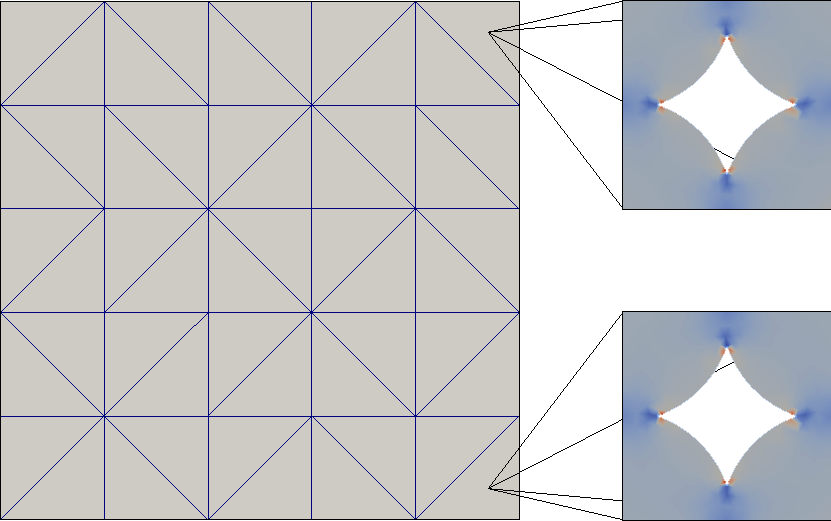
\includegraphics[width=0.9\textwidth]{figures/Sintering_5x5_000.png}\\
 $\longrightarrow$\\[0.5em]
 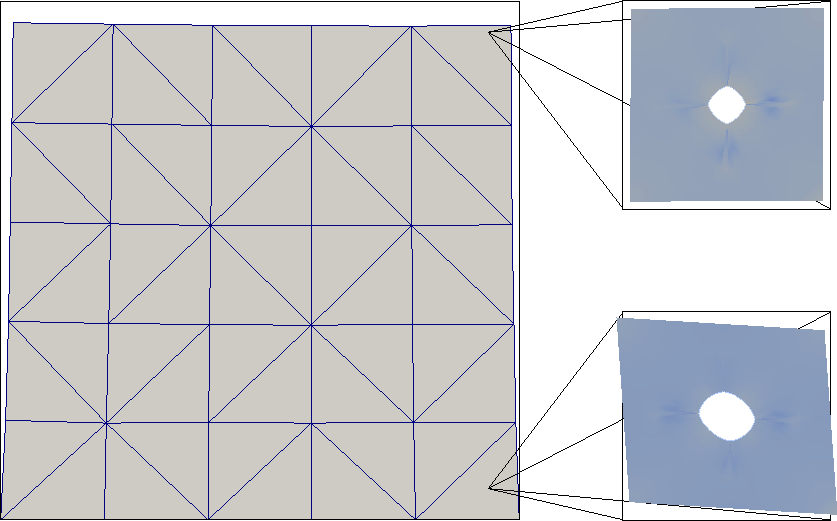
\includegraphics[width=0.9\textwidth]{figures/Sintering_5x5_114.png}
\end{center}
\end{columns}
\end{frame}

\subsubsection{Results}
\begin{frame}
 \frametitle{Numerical results}
\begin{center}
\movie[height=6cm,width=9.7cm,poster]{}{Sintering_5x5.avi}

\movie[externalviewer]{Multiscale sintering}{Sintering_5x5.mpeg}
\end{center}
\end{frame}

\section{Implementation}
\subsection{OOFEM}
\begin{frame}
 \frametitle{OOFEM -- Finite element }
 Implementation
 \begin{enumerate}
  \item Implementing constitutive drivers for macroscale
  \item Subscale is just another FE problem
  \item Some difficulties fitting into the design of OOFEM
 \end{enumerate}

\onslide<2-> Some positive notes
 \begin{enumerate}
  \item<2-> Parallel computations: Already designed for message passage paradigm.
  \item<2-> Nonlinear solvers
  \begin{itemize}
   \item<2-> Several linear solvers
   \item<2-> Line-search solvers
   \item<2-> Newton solvers
  \end{itemize}
  \item<2-> Exporting data
  \item<2-> Adaptivity
  \item<2-> Cooperation, \url{http://www.oofem.org/}
 \end{enumerate}

\end{frame}

\section{Future}
\begin{frame}
 \frametitle{Future work}
 Requirements for realistic microstructures
 \begin{enumerate}
  \item Remeshing
  \begin{itemize}
   \item Levelset representation of voids and particles
   \item Multiple surfaces
   \item Vanishing pores
  \end{itemize}
  \item 3D
 \end{enumerate}
 Other work
 \begin{enumerate}
  \item Weakly periodic boundary conditions (Neumann boundary condition as special case)
  \item Comparison against macroscopic experiments.
 \end{enumerate}

\end{frame}

% \section{End of presentation}
% \begin{frame}
%  \frametitle{Thank you!}
%  \nocite{*}
%  \printbibliography{}
% \end{frame}


\end{document}
